\documentclass{beamer}
\usepackage{etex}
\usetheme{Boadilla}
\usepackage{tikz}
\usepackage{tikz-qtree}
\usepackage{lmodern}
\usepackage{fancybox}
\usepackage{calc}
\usepackage{amsfonts,amssymb, mathrsfs, amsmath}
\usepackage{color}
\usepackage[color,matrix,arrow,all]{xy}


\title{Concepts, Definitions, and Inheritance}
\subtitle{Interpreting the atoms of lexical decomposition}
\author{David Zornek}
\institute[CMU]{
  Department of Philosophy\\
  Carnegie Mellon University\\
  \texttt{dzornek@andrew.cmu.edu}
}
\date{May 1, 2013}

\begin{document}

\begin{frame}[plain]
  \titlepage
\end{frame}

\begin{frame}{Decompositional Semantics}
\begin{columns}
 \column{0.8\textwidth}
``But, we can know the Markerese translation of an English sentence without knowing the first thing about the meaning of the English sentence... Translation into Markerese is at best a substitute for real semantics, relying either on our tacit competence (at some future date) as speakers of Markerese or on our ability to do real semantics at least \\ for the one language Markerese.''
\par\vspace{.25in}
\hfill -David Lewis, ``General semantics'' (1970)
\end{columns}
\end{frame}

\begin{frame}{Outline}
\begin{columns}
 \column{0.8\textwidth}
\begin{enumerate}
\item Decompositional Semantics
\vspace{.125in}
\item Concepts
\vspace{.125in}
\item Inheritance Networks
\vspace{.125in}
\item The Genus-differentia Inheritance Theorem (GDIT)
\vspace{.125in}
\item Practical Consequences for Cognitive Science
\vspace{.125in}
\item Steps for future research
\end{enumerate}
\end{columns}
\end{frame}

\begin{frame}{Decompositional Semantics}
\begin{columns}
 \column{0.8\textwidth}
``But, we can know the Markerese translation of an English sentence without knowing the first thing about the meaning of the English sentence... Translation into Markerese is at best a substitute for real semantics, relying either on our tacit competence (at some future date) as speakers of Markerese or on our ability to do real semantics at least \\ for the one language Markerese.''
\par\vspace{.25in}
\hfill -David Lewis, ``General semantics'' (1970)
\end{columns}
\end{frame}

\begin{frame}{Decompositional Semantics}
\begin{columns}
 \column{0.8\textwidth}
``But, we can know the Markerese translation of an English sentence without knowing the first thing about the meaning of the English sentence... Translation into Markerese is at best a substitute for real semantics, relying either on our {\bf tacit competence} (at some future date) as speakers of Markerese or on our ability to do real semantics at least \\ for the one language Markerese.''
\par\vspace{.25in}
\hfill -David Lewis, ``General semantics'' (1970)
\end{columns}
\end{frame}

\begin{frame}{Decompositional Semantics}
\begin{columns}
 \column{0.8\textwidth}
``But, we can know the Markerese translation of an English sentence without knowing the first thing about the meaning of the English sentence... Translation into Markerese is at best a substitute for real semantics, relying either on our {\bf tacit competence} (at some future date) as speakers of Markerese or on our ability to do {\bf real semantics at least for the one language Markerese}.''
\par\vspace{.25in}
\hfill -David Lewis, ``General semantics'' (1970)
\end{columns}
\end{frame}

\begin{frame}{Real Semantics for Markerese}
\begin{columns}
 \column{0.8\textwidth}
Some guiding intuitions about real semantics:
\par\vspace{.125in}
\begin{enumerate}
\item It must explain/capture the sense of aboutness.
\vspace{.125in}
\item It must admit of empirical inquiry.
\vspace{.125in}
\item It cannot be a reduction to some other formal language, which we will take to mean:
\vspace{.125in}
\item It will take the form of interpreting Markerese as some real-world phenomenon.
\end{enumerate}
\uncover<2->{
	\begin{block}{Proposal}
	Interpret semantic atoms as concepts.
	\end{block}
	}
\end{columns}
\end{frame}

\begin{frame}{The Classical View of Concepts: \\ Genus-Differentia Definitions}
\begin{columns}
 \column{0.8\textwidth}
\begin{enumerate}
	\item A full analysis of a concept is given by a genus-differentia definition.
\par\vspace{.125in}
\quad \emph{Example:} human := rational animal
\par\vspace{.125in}
\quad\quad\quad\quad $\bullet$ genus: animal
\par
\quad\quad\quad\quad $\bullet$ differentia: rational
\end{enumerate}
\end{columns}
\end{frame}

\begin{frame}{The Classical View of Concepts: \\ Genus-Differentia Definitions}
\begin{columns}
 \column{0.8\textwidth}
What constitutes a ``full analysis''?
\par\vspace{.125in}
\begin{description}
\item[(I)] Definitions specify what is \emph{intrinsic} to a concept, by virtue of their stipulation of necessary and sufficient conditions for category membership, and
\item[(R)] Definitions specify a hierarchy relation that holds between concepts, which \emph{relates} a concept to others within a hierarchy.
\end{description}
\end{columns}
\end{frame}

\begin{frame}{The Classical View of Concepts: \\ Its Downfall}
\begin{columns}
 \column{0.8\textwidth}
\begin{enumerate}
\item Wittgenstein argued for family resemblances, rather than definitions, determine category membership.
\vspace{.25in}
\item Beginning with Rosch's experiments, empirical research has validated Wittgenstein's result.
\par\vspace{.125in}
\quad\quad \emph{Example:} Brain-dead humans are not rational.
\par\vspace{.125in}
\uncover<2->{
	Important: This only refutes (I), and there is reason to believe that (R) is true.
}

\end{enumerate}
\end{columns}
\end{frame}

\begin{frame}{Concepts: Hierarchical Organization}
\begin{columns}
 \column{0.8\textwidth}
\begin{enumerate}
	\item Rosch's experiments also showed that concepts are organized hierarchically.
\vspace{.125in}
	\item Genus-differentia definitions do serve as a set of coordinates that locate a concept within the hierarchy.
\end{enumerate}
\end{columns}
\end{frame}

\begin{frame}{Conceptual Hierarchy}
\centerline{
\xymatrix{
& \textbf{animal} & \\
\textbf{rational} \ar[ur] & & \textbf{language-using} \ar[ul] \\
& \textbf{human} \ar[ur] \ar[ul] & \\
\textbf{adult\_male} \ar[ur] \ar@{--}[rr] & & \textbf{adult\_female} \ar[ul]  }
}
\end{frame}

\begin{frame}{Inheritance Networks}
\centerline{
\xymatrix{
& \textbf{animal} & \\
\textbf{rational} \ar[ur] & & \textbf{language-using} \ar[ul] \\
& \textbf{human} \ar[ur] \ar[ul] & \\
\textbf{adult\_male} \ar[ur] \ar@{--}[rr] & & \textbf{adult\_female} \ar[ul]  }
}
\end{frame}

\begin{frame}{Inheritance Networks vs. Conceptual Hierarchy}
\begin{center}
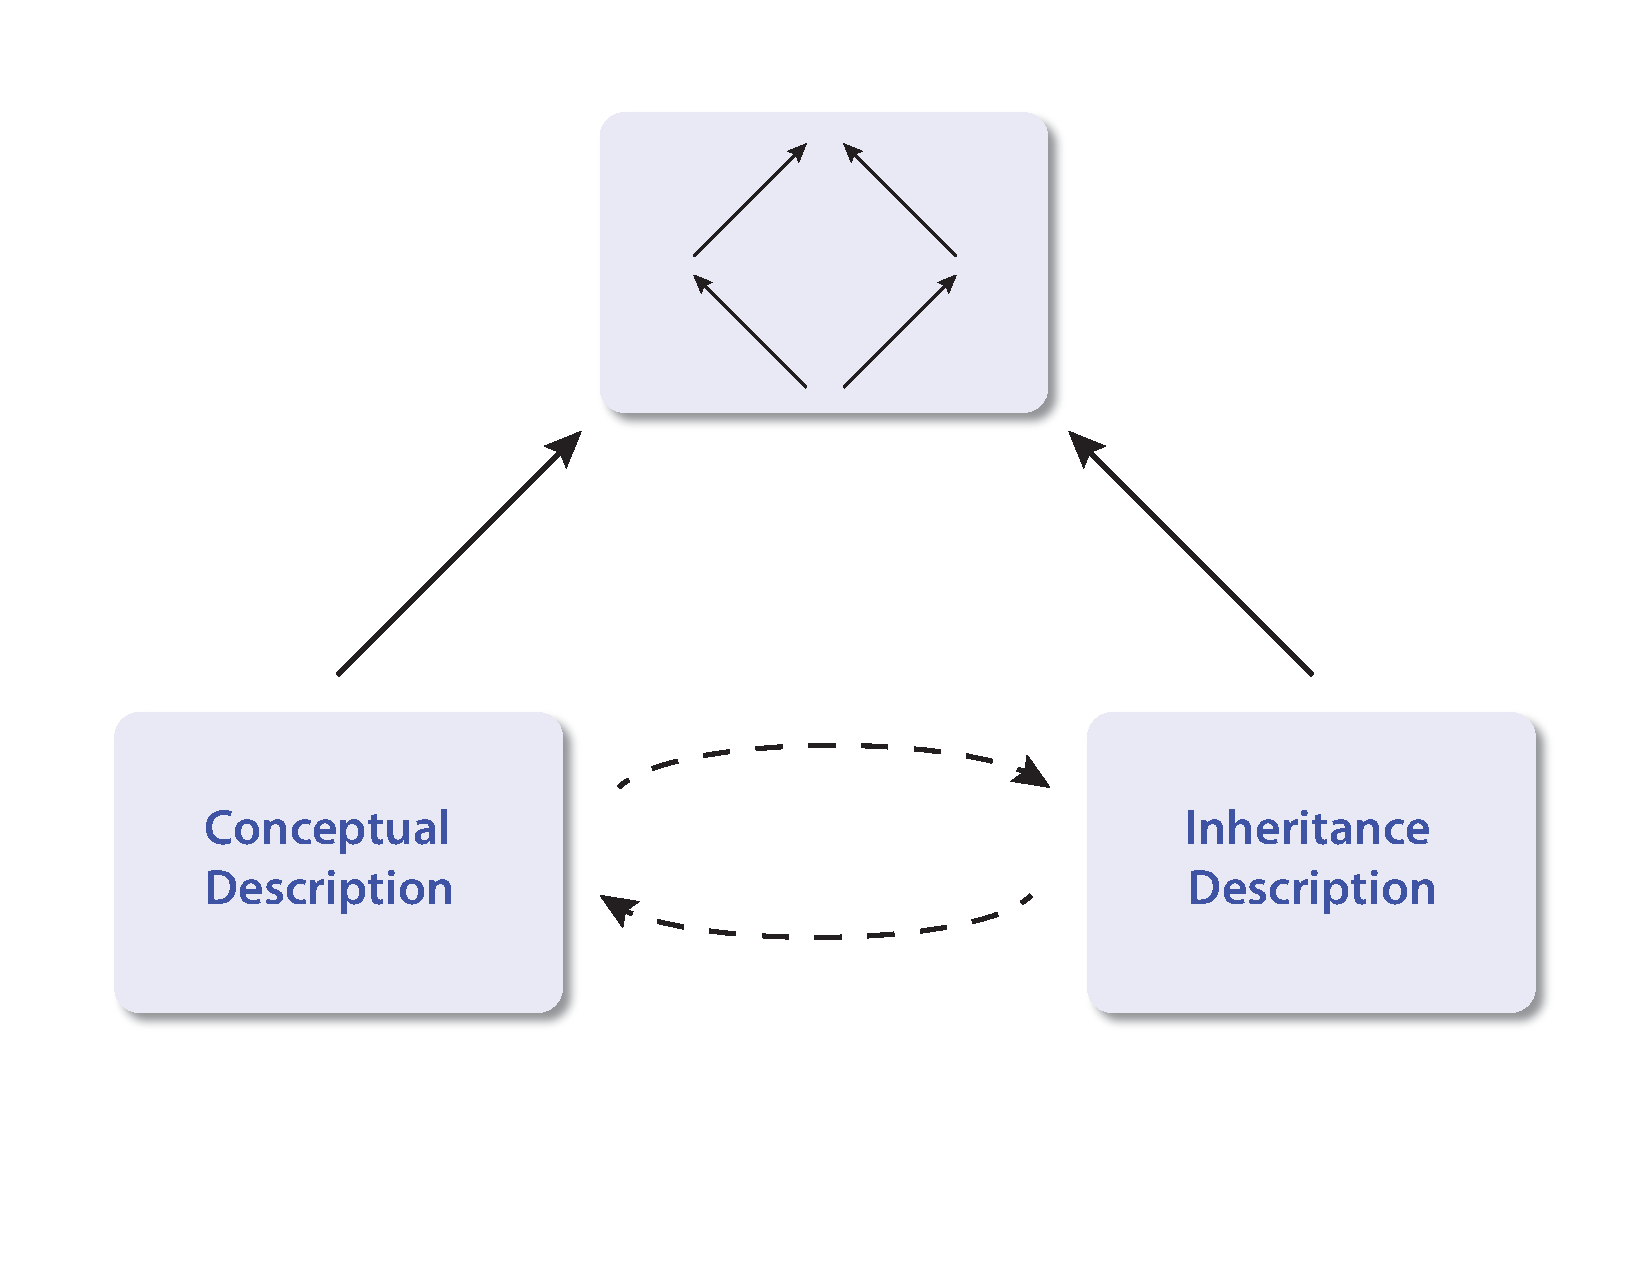
\includegraphics[width=4in]{InheritanceVsConcepts_1}
\end{center}
\end{frame}

\begin{frame}{Inheritance Networks vs. Conceptual Hierarchy}
\begin{center}
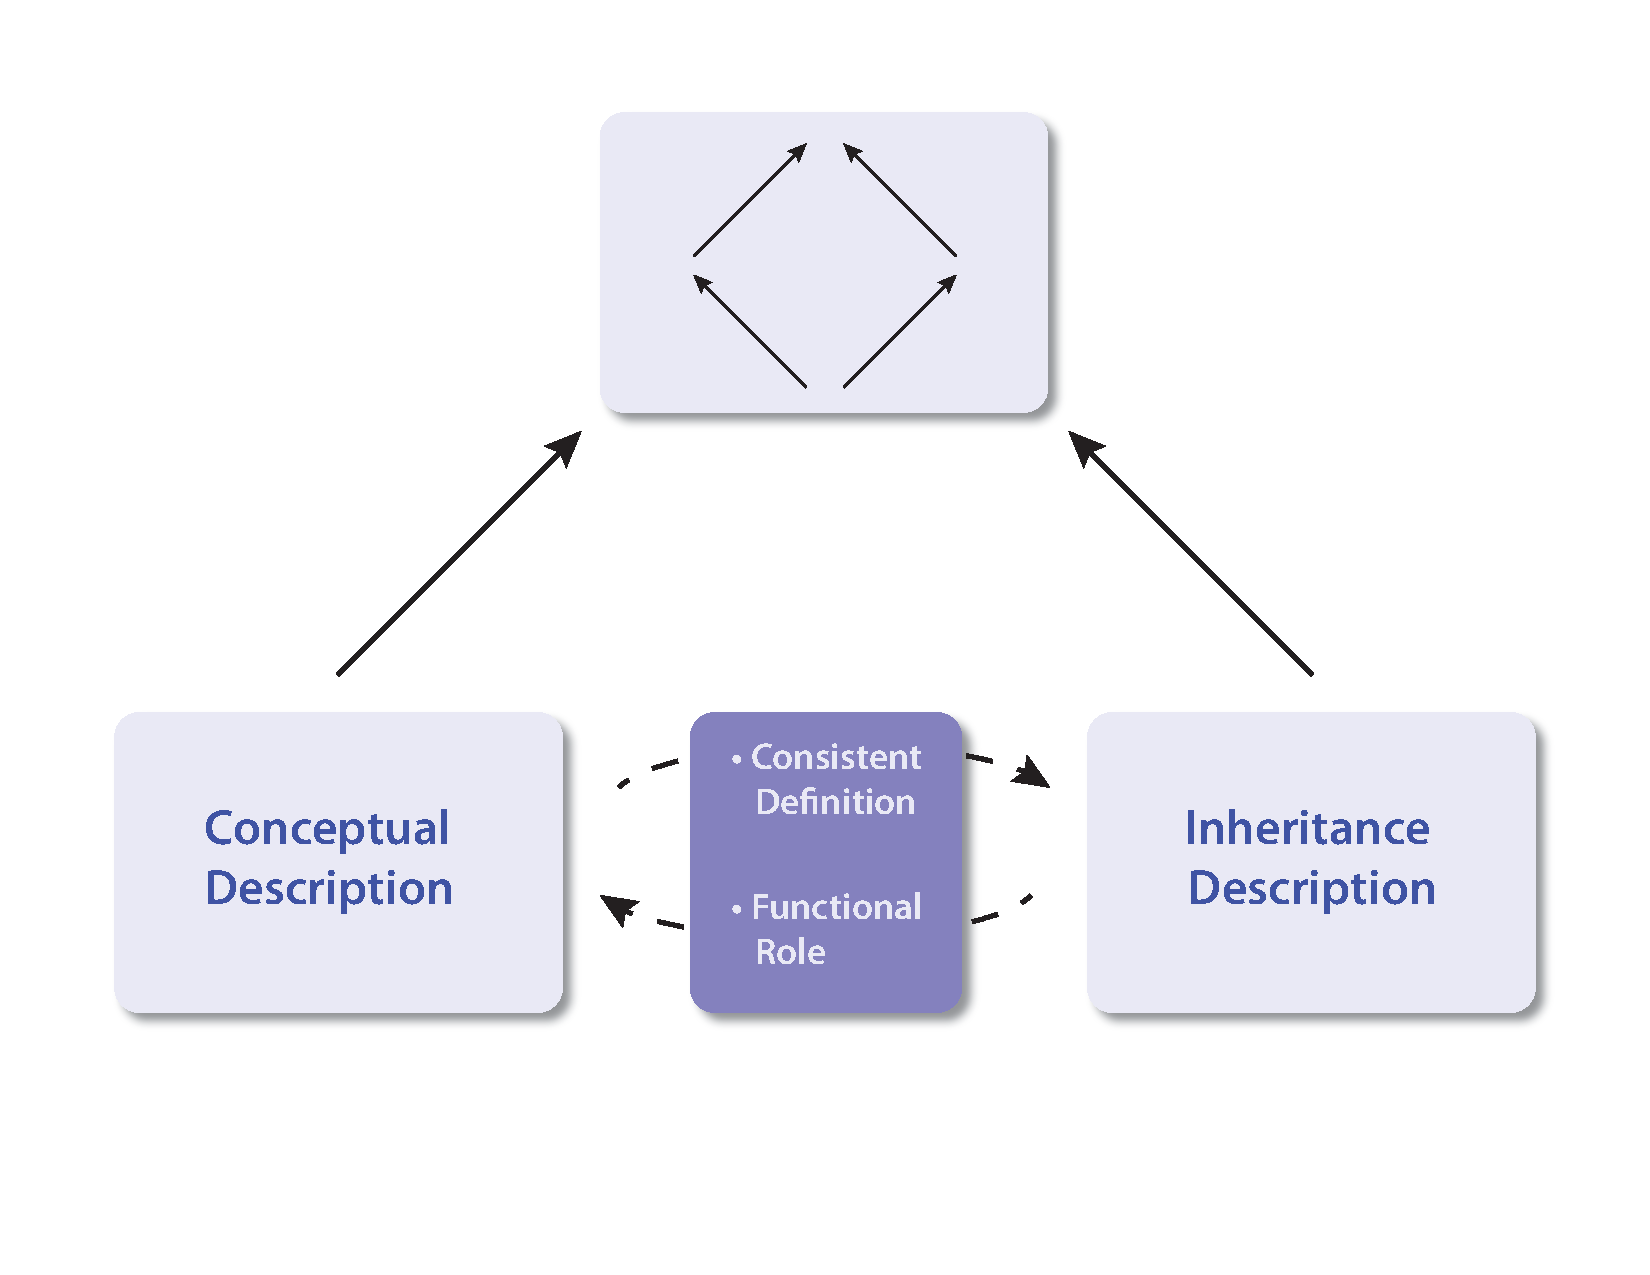
\includegraphics[width=4in]{InheritanceVsConcepts_2}
\end{center}
\end{frame}

\begin{frame}{Inheritance Networks - Consistent Definition}
\centerline{
\xymatrix{
& \textbf{animal} & \\
\textbf{rational} \ar[ur] & & \textbf{language-using} \ar[ul] \\
& \textbf{human} \ar[ur] \ar[ul] & \\
\textbf{adult\_male} \ar[ur] \ar@{--}[rr] & & \textbf{adult\_female} \ar[ul]  }
}
\vspace{.25in}
$$D_{\textbf{human},1}=\{\textbf{human},\textbf{rational},\textbf{animal}\}$$
$$D_{\textbf{human},2}=\{\textbf{human},\textbf{language-using},\textbf{animal}\}$$
\end{frame}

\begin{frame}{Inheritance Networks - Consistent Definition}
\centerline{
\xymatrix{
& \textbf{animal} & \\
\textbf{rational} \ar[ur] & & \textbf{language-using} \ar[ul] \\
& \textbf{human} \ar[ur] \ar[ul] & \\
\textbf{adult\_male} \ar[ur] \ar@{--}[rr] & & \textbf{adult\_female} \ar[ul]  }
}
\vspace{.25in}
$$D_{\textbf{man},1}=\{\textbf{adult\_male},\textbf{human},\textbf{rational},\textbf{animal}\}$$
$$D_{\textbf{man},2}=\{\textbf{adult\_male},\textbf{human},\textbf{language-using},\textbf{animal}\}$$
\end{frame}

\begin{frame}{Inheritance Networks - Functional Role}
\centerline{
\xymatrix{
& \textbf{animal} & \\
\textbf{rational} \ar[ur] & & \textbf{language-using} \ar[ul] \\
& \textbf{human} \ar[ur] \ar[ul] & \\
\textbf{adult\_male} \ar[ur] \ar@{--}[rr] & & \textbf{adult\_female} \ar[ul]  }
}
\vspace{.25in}
$$i(\textbf{human})=\{D_{\textbf{human},1},D_{\textbf{human},2},D_{\textbf{man},1},D_{\textbf{man},2},D_{\textbf{woman},1},D_{\textbf{woman},2}\}.$$
$$i(\textbf{adult\_male})=\{D_{\textbf{man},1},D_{\textbf{man},2}\}.$$
\end{frame}

\begin{frame}{The GDIT}
\begin{columns}
 \column{0.8\textwidth}
\begin{block}{Genus-differentia Inheritance Theorem}
$i(\alpha)\subseteq i(\beta)\Leftrightarrow \alpha\sqsubseteq\beta$
\end{block}
\vspace{.25in}
\begin{itemize}
\item Inheritance relation: $\sqsubseteq$
\item Semantic atoms/concepts: $\alpha,\beta$
\item Functional roles: $i(\alpha),i(\beta)$
\end{itemize}
\end{columns}
\end{frame}


\begin{frame}{The GDIT}
\begin{columns}
 \column{0.8\textwidth}
\begin{block}{Genus-differentia Inheritance Theorem}
Inheritance networks, semantic content, and conceptual hierarchy are isomorphic to each other.
\end{block}
\vspace{.125in}
\begin{itemize}
\item The functional role is a partial set of identity conditions for semantic content and concepts.
\vspace{.125in}
\item If $\alpha$ and $\beta$ are the same concept, then they are located at the same position in the hierarchy.
\end{itemize}
\vspace{.25in}
\end{columns}
\end{frame}

\begin{frame}{Practical Consequences for Cognitive Science: \\ A puzzle about concepts}
\begin{columns}
 \column{0.8\textwidth}
\begin{center}
Test Sentence: ``He began the novel.''
\end{center}
\end{columns}
\end{frame}

\begin{frame}{Practical Consequences for Cognitive Science}
$$\left[
\begin{array}{l l}
\textbf{novel} & \\
\text{ARG}_1 = & \textbf{x:book} \\
\text{QUALIA} = & \left[ \begin{array}{l}
				\text{CONST}=\textbf{narrative(x)} \\
				\text{FORMAL}=\textbf{book(x)} \\
				\text{TELIC}=\textbf{read(x)} \\
				\text{AGENT}=\textbf{write(x)}
				\end{array}\right] \\
\end{array}
\right]$$
\vspace{.125in}
$$\left[
\begin{array}{l l}
\textbf{begin} & \\
\mathcal{A} = & \left[ \begin{array}{l}
	\text{ARG}_1=\textbf{animate\_obj} \\
	\text{ARG}_2=\textbf{event}_1 \\
	\end{array}\right] \\
\mathcal{E} = & \left[ \begin{array}{l}
	\text{E}_1=\textbf{transition} \\
	\mathellipsis \\
	\end{array}\right] \\
\mathcal{Q} = &  \left[ \begin{array}{l}
	\text{FORMAL}=\textbf{P(event}_1\textbf{,x)} \\
	\text{AGENT} = \textbf{begin\_act(event}_1\textbf{,x}\textbf{)} \\
	\end{array}\right] \\
\end{array}
\right]$$
\end{frame}

\begin{frame}{Practical Consequences for Cognitive Science}
\begin{center}
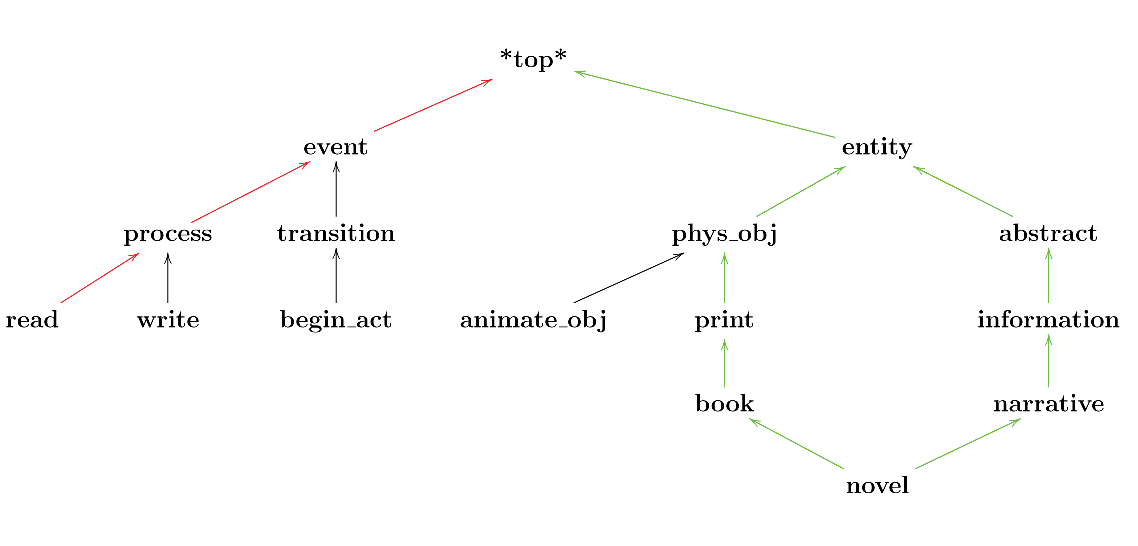
\includegraphics[width=4.75in]{InheritanceNetwork}
\end{center}
\end{frame}


\begin{frame}{Areas for Future Research}
\begin{columns}
 \column{0.8\textwidth}
\begin{enumerate}
\item Can we learn about inheritance by looking at linguistics and/or concepts?
\vspace{.125in}
\item Adding relations to the partial order
\vspace{.125in}
\item Can we arrive at a sufficient condition for identity between concepts?
\end{enumerate}
\end{columns}
\end{frame}

\begin{frame}
\begin{center}
Thank you!
\end{center}
\end{frame}

\begin{frame}{Formal definitions}
\noindent{\bf (Inheritance Network)} An \normalfont{inheritance network} $\mathcal{I}$ is a triple $\langle\mathcal{B},\sqsubseteq,\#\rangle$ where:
\begin{itemize}
\item $\mathcal{B}$ is a finite set of \normalfont{basic elements}
\item $\sqsubseteq\subseteq\mathcal{B}\times\mathcal{B}$ is the basic \emph{inheritance} relation
\item $\#\subseteq\mathcal{B}\times\mathcal{B}$ is the basic \emph{disjointness} relation
\end{itemize}
\par\vspace{5mm}
\noindent{\bf (Inheritance/Disjointness)} The \emph{inheritance} relation $\sqsubseteq^*\subseteq\mathcal{B}\times\mathcal{B}$ is the smallest such that:
\begin{itemize}
\item $P\sqsubseteq^*P$  (Reflexivity)
\item if $P\sqsubseteq Q$ and $Q\sqsubseteq^*R$ then $P\sqsubseteq^*R$ (Transitivity)
\end{itemize}
The \emph{disjointness} relation $\#^*\subseteq\mathcal{B}\times\mathcal{B}$ is the smallest such that:
\begin{itemize}
\item if $P\#Q$ or $Q\#P$ then $P\#^*Q$ (Symmetry)
\item if $P\sqsubseteq^*Q$ and $Q\#^*R$ then $P\#^*R$ (Chaining)
\end{itemize}
\end{frame}

\begin{frame}{Formal definitions}
\noindent{\bf (Consistent Definition)} A set $D\subseteq\mathcal{B}$ is a \emph{consistent definition} for $\mathcal{B}$ iff:
\begin{enumerate}
\item For all $x,y\in D$, it is not the case that $x\#y$.
\item For all $x\in D$, $y_1,\mathellipsis,y_n\in\mathcal{B}$, if $x\sqsubseteq y_i$, then $y_i\in D$ iff there is no $y_j\in D$ such that neither $y_i\sqsubseteq y_j$ nor $y_j\sqsubseteq y_i$.
\item There exists an $\alpha_b$ (called the \emph{base atom} or \emph{base} of $D$), such that for all $y_1,\mathellipsis,y_n\in\mathcal{B}$, if $y_i\sqsubseteq \alpha_b$, then $y_i\notin D$, i.e. $D$ has a minimal element.
\end{enumerate}
\par\vspace{5mm}
\noindent {\bf (Funtional Role)}. The \emph{functional role} of an an atom is a function $i:\mathcal{B}\rightarrow\mathcal{F})$ such that
$$i(x)=\{D\in\mathcal{F}\vert x\in D\},$$
where $\mathcal{F}$ is the set of all consistent definitions $D$ on $\mathcal{B}$.
\end{frame}

\begin{frame}{Formal definitions}
\begin{columns}
\column{0.8\textwidth}
\begin{block}{Genus-differentia Inheritance Theorem}
 Given $\sqsubseteq $ and $\#$,  such that $\sqsubseteq $ is inclusion and $\#$ is disjointness over $\mathcal{B}$, a consistently definable set of atoms, there exists a non-empty functional role $i$ such that $a\sqsubseteq b\Leftrightarrow i(a)\subseteq i(b)$  and $a\#b\Leftrightarrow i(a)\cap i(b)=\emptyset$.
\end{block}
\end{columns}
\end{frame}

\begin{frame}{Proof of the GDIT - Lemma 3.1}
\begin{columns}
\column{0.8\textwidth}
\begin{block}{Lemma 3.1}
For $a,b\in\mathcal{B}$ such that it is not the case that $a\#b$, let $D_a=\{c\vert a\sqsubseteq c\}$ and $D_b=\{c\vert b\sqsubseteq c\}$. $D^*=D_a\cup D_b$ is a consistent definition on $\mathcal{B}$.
\end{block}
Proof. Because of the reflexivity of $\sqsubseteq$, it is obvious that  $D^*$ meets condition (2) above. Suppose (1) does not hold of $D^*$, i.e. there exists $x,y\in D^*$ such that $x\#y$. Then, by chaining we know that $a\#b$, since for all $x\in D^*$, either $a\sqsubseteq x$ or $b\sqsubseteq x$. But we have already said that it is not the case that $a\#b$, so (1) must hold of $D^*$. Therefore $D^*$ is a consistent definition on $\mathcal{B}$. \hfill $\openbox$
\end{columns}
\end{frame}

\begin{frame}{Proof of the GDIT - Lemma 3.2}
\begin{columns}
\column{0.8\textwidth}
\begin{block}{Lemma 3.2}
Let $a,b\in\mathcal{B}$ be such that it is not the case that $a\sqsubseteq b$, and let $\mathcal{F}=\{D\vert D\text{ is a consistent definition}\}$. If $a$ is consistently definable, then there exists some $D_{\lnot b}^a\in\mathcal{F}$ such that $a\in D_{\lnot b}^a$ and $b\notin D_{\lnot b}^a$.
\end{block}

Proof. Assume $a$ is consistently definable. Then there exists some $D^a\in\mathcal{F}$ such that $a\in D^a$. Either $a\# b$ or not. Suppose $a\#b$. Then $b\notin D^a$, by condition (1) for consistent definition. Suppose it is not the case that $a\#b$. Then there is no relation between $a$ and $b$, which means that if $D^a$ is a consistent definition, then $D_{\lnot b}^a=D^a\setminus\{b\}$ is also a consistent definition. By the definition of $D_{\lnot b}^a$, $b\notin D_{\lnot b}^a$ and $a\in D_{\lnot b}^a$. \hfill $\openbox$
\end{columns}
\end{frame}

\begin{frame}{Proof of the GDIT}
Let $\mathcal{F}=\{D\vert D\text{ is a consistent definition on }\mathcal{B}\}$, and let $i:\mathcal{B}\rightarrow\mathcal{P}(\mathcal{F})$ be a function such that $i(x)=\{D\in\mathcal{F}\vert x\in D\}$.
\par\vspace{.125in}
Assume $a\sqsubseteq b$. Suppose $D\in i(a)$. Then $a\in D$, by the definition of $i$, which means that $b\in D$ by (2). So $D\in i(b)$, by the definition of $i$. We therefore have $a\sqsubseteq b\Rightarrow i(a)\subseteq i(b)$.
\par\vspace{.125in}
Assume that it is not the case that $a\sqsubseteq b$. Then, by (3.2) there exists some $D^a_{\lnot b}\in\mathcal{F}$ such that $a\in D^a_{\lnot b}$ and $b\notin D^a_{\lnot b}$. Then $D^a_{\lnot b}\in i(a)$, but $D^a_{\lnot b}\notin i(b)$, which means that $i(a)\not\subseteq i(b)$. So we have: If it is not the case that $a\sqsubseteq b$, then it is not the case that $i(a)\subseteq i(b)$, which contraposits to $i(a)\subseteq i(b)\Rightarrow a\sqsubseteq b$.
\par\vspace{.125in}
We have therefore shown that $a\sqsubseteq b\Leftrightarrow i(a)\subseteq i(b)$, and we now turn to proving that $a\#b\Leftrightarrow i(a)\cap i(b)=\emptyset$.
\end{frame}

\begin{frame}{Proof of the GDIT}
Assume $a\#b$. Now suppose $i(a)\cap i(b)\neq\emptyset$. Then there exists some $D\in\mathcal{F}$ such that $a\in D$ and $b\in D$. But, by (1), this cannot be the case. So,  $a\#b\Rightarrow i(a)\cap i(b)=\emptyset$.
\par\vspace{.125in}
Assume $i(a)\cap i(b)=\emptyset$. Then there exists no $D\in\mathcal{F}$ such that $a\in D$ and $b\in D$. Now suppose it is not the case that $a\#b$. Let $D_a$, $D_b$, and $D^*$ be defined as in (3.1). Then  $D^*$ is a consistent definition on $\mathcal{B}$. But, by the reflexivity of $\sqsubseteq $, $a\in D_a$ and $b\in D_b$, which means that $a,b\in D^*$. So there is some $D\in\mathcal{F}$ such that $a\in D$ and $b\in D$, a contradiction. Therefore, $i(a)\cap i(b)=\emptyset\Rightarrow a\#b$.
\par\vspace{.125in}
We have therefore shown that $i(a)\cap i(b)=\emptyset\Leftrightarrow a\#b$.
\end{frame}
\end{document}